\documentclass[dvipdfmx]{jsarticle}
\usepackage[dvipdfmx]{graphicx}
\usepackage{amsmath,amssymb,amsfonts,amsthm,enumerate}
\usepackage{float}
\usepackage{bm}
\usepackage{multirow}
\usepackage{hhline}
\usepackage{diagbox}
\usepackage{caption}
\usepackage{algorithm}
\usepackage{algpseudocode}
\usepackage{colortbl}
\usepackage[subrefformat=parens]{subcaption}
\captionsetup{compatibility=false}

\setlength\floatsep{0pt} %dblfloatsep

\newcommand{\argmax}{\mathop{\rm arg~max}\limits}
\newcommand{\argmin}{\mathop{\rm arg~min}\limits}

\newenvironment{hangall}[1]{\hangindent = #1zw\everypar{\hangindent = #1zw}}{}

\setlength{\topmargin}{-25mm}
\setlength{\textheight}{270mm}
\setlength{\oddsidemargin}{-10mm}
\setlength{\textwidth}{170mm}

\bibliographystyle{jplain}
\begin{document}

\begin{center}
  \begin{tabular}[h]{|c|c|c|c|c|c|c|c|}
    \multicolumn{8}{l}{}                                                                          \\
    \hline
    \multicolumn{7}{|c|}{\begin{minipage}{120mm}\vspace{.2zh}TITLE\\[-3.1zh]\begin{center}
          %%%%%%%%%%%%%%%%%%%%%%%%%%%%%%%%%%%%%%%%%%
          関連研究の調査と今後の計画
          %%%%%%%%%%%%%%%%%%%%%%%%%%%%%%%%%%%%%%%%%%
        \end{center}\end{minipage}}
     & \begin{minipage}{20mm}Rep-No.\\[-.5zh]\hspace{3.5em}
         %%%%%%%%%%%%%%%%%%%%%
         3
         %%%%%%%%%%%%%%%%%%%
       \end{minipage}                                        \\\hline
    \multicolumn{8}{|c|}{\begin{minipage}{120mm}\vspace{.2zh}AFFILIATION\\[-3.1zh]\begin{center}
          %%%%%%%%%%%%%%%%%%%%%%%%%%%%%%%%%%%%%%%%%%
          九州大学大学院 システム情報科学府 鈴木研究室
          %%%%%%%%%%%%%%%%%%%%%%%%%%%%%%%%%%%%%%%%%%
        \end{center}\end{minipage}}
    \\\hline
    \multicolumn{3}{|c}{\begin{minipage}{60mm}\vspace{.2zh}AUTHOR\\[-.7zh]
                            \hspace{7em}Ichinose Haruki\end{minipage}}
     & \multicolumn{2}{|r}{\begin{minipage}{40mm}POSITION\\[-.7zh]\hspace{7.5em}B4\end{minipage}}
     & \multicolumn{3}{|c|}{\begin{minipage}{60mm}DATE\\[-.7zh]\hspace{9em}
                                %%%%%%%%%%%%%%%%%%%%%%%%%%%%%%%%%%%%%
                                2025/06/24
                                %%%%%%%%%%%%%%%%%%%%%%%%%%%%%%%%%%%%%

                              \end{minipage}}                        \\\hline
  \end{tabular}
\end{center}

\section{前回の発表について}

前回の発表では, LLMを用いて, 統計データとその偏見的説明文から, それに対する効果的な対抗説明文を生成する手法の提案を行った.
この手法は, 以下の2つのフェーズから構成されていた.

\begin{itemize}
  \item フェーズ1: SelectInstinctによる本能の特定
  \item フェーズ2: LLMによる対抗文生成
\end{itemize}

\vspace{1em}

\section{関連研究:Towards Knowledge-Grounded Counter Narrative Generation for Hate Speech \cite{chung2021}}

本研究は, ヘイトスピーチ(HS)に対抗するカウンターナラティブ(CN)の自動生成において, 従来の生成モデルが抱える具体性・根拠の欠如やハルシネーションといった課題を解決することを目的としている.
そのために, Wikipediaやニュース記事などの外部知識に基づいて, より情報量が多く説得力のあるCNを生成する, 初の包括的パイプラインを提案した.

\subsection{論文情報}
\begin{itemize}
  \item \textbf{タイトル}: Towards Knowledge-Grounded Counter Narrative Generation for Hate Speech
  \item \textbf{著者}: Yi-Ling Chung, Serra Sinem Tekiroğlu, Marco Guerini
  \item \textbf{発表年}: 2021年
  \item \textbf{公開}: Findings of the Association for Computational Linguistics: ACL-IJCNLP 2021
  \item \textbf{被引用数}: 78
\end{itemize}

\vspace{0.5em}

\subsection{背景と課題}

\begin{itemize}
  \item \textbf{HS対策とCNの現状}
        \begin{itemize}
          \item 現在, HS対策としてコンテンツ削除やシャドウバンなどが主に行われているが, 言論の自由や多様性の観点から懸念も存在する.
          \item 事実に基づいた議論や異なる視点による反論としてCNが注目されている.
        \end{itemize}

  \item \textbf{効果的なCNの例}
        \begin{figure}[H]
          \centering
          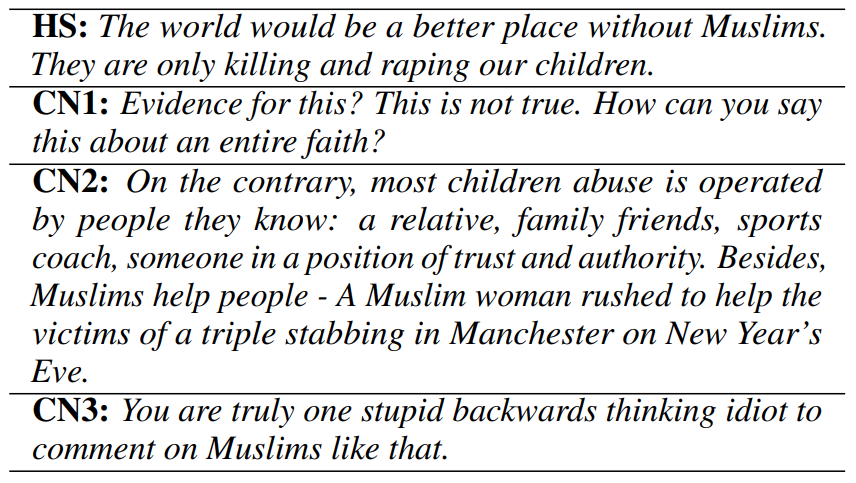
\includegraphics[width=0.6\textwidth]{01.png}
          \caption{HSに対する適切なCN(CN1, CN2)および不適切なCN(CN3)の例 \cite{chung2021}}
          \label{fig:cn_example}
        \end{figure}
        \begin{itemize}
          \item CN1とCN2はいずれも適切だが, CN2は事実や知識, 論理的推論に基づいており, より説得力が高い.
          \item CN3は攻撃的で不適切な応答である.
        \end{itemize}
\end{itemize}

\vspace{0.5em}

\subsection{HS-CNデータセット}

\begin{itemize}
  \item \textbf{データセット}: CONAN
  \item \textbf{特徴}: NGOの専門家によって作成されており, 高品質
  \item \textbf{データ数}: 6,645組(パラフレーズして作成したものや仏・伊語からの翻訳を含む)
  \item \textbf{分割}:
        \begin{itemize}
          \item 訓練: 4,069組
          \item 開発: 1,288組
          \item テスト: 1,288組
        \end{itemize}
\end{itemize}

この研究では, リバースエンジニアリングを用いて, 既存データセットに知識を検索・付与する方法で新たなデータセットを構築している.

\vspace{0.5em}

\subsection{提案手法}

本研究は, 外部知識に基づいたCNを生成するため, 以下に示す2段階の構成のアーキテクチャを提案している.

\subsubsection{知識検索モジュール(Knowledge Retrieval)}

与えられたHSに対して, CNの根拠となる知識を外部リポジトリから検索・抽出する.

\begin{itemize}
  \item \textbf{知識ソース}:
        \begin{itemize}
          \item Newsroom(130万件以上のニュース記事)
          \item WikiText-103(28,595件のWikipedia記事)
        \end{itemize}
        \vspace{0.5em}

  \item \textbf{クエリ構築法}: 関連知識を検索するためのキーワード(クエリ)を構築する.
        \begin{enumerate}
          \item \textbf{抽出型(Extraction)}: 訓練時には, HSと正解CNの両方からキーフレーズを抽出し, 検索精度を高める.
          \item \textbf{生成型(Generation)}: テスト時には正解CNが利用できないため, HSを入力として, 反論に有効なキーフレーズを予測・生成するAIモデルを別途用意する.
        \end{enumerate}
        \vspace{0.5em}

  \item \textbf{知識選定}:
        クエリを用いて関連文書を検索後, 各文とクエリの関連度(ROUGE-Lスコア)を計算し, 最も関連性の高い上位5文を知識文(KN)として選定し, 生成モジュールに入力する.
\end{itemize}

\vspace{0.5em}

\subsubsection{CN生成モジュール(Counter Narrative Generation)}

\begin{itemize}
  \item \textbf{入力}: 元のHSおよび検索された知識文(KN)
  \item \textbf{モデル}: GPT-2などの大規模言語モデルをファインチューニングし, 与えられた知識を反映させながらCNを生成する.
        本研究では特にGPT-2モデルを重点的に評価している.
\end{itemize}

\begin{figure}[H]
  \centering
  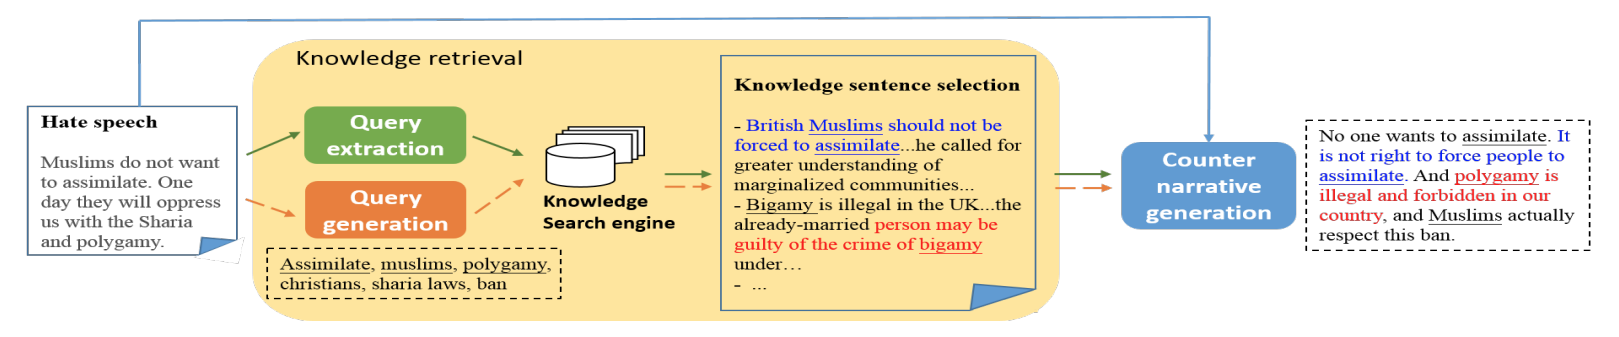
\includegraphics[width=1.0\textwidth]{02.png}
  \caption{抽出型(緑の実線矢印)と生成型(点線矢印)のクエリを用いて関連知識を検索する, 知識文に基づいた生成アーキテクチャ\cite{chung2021}}
  \label{fig:architecture}
\end{figure}

\vspace{0.5em}

\subsection{実験と結果}

BLEU-2やROUGE-Lを用いた自動評価と, NGOの専門家による手動評価の2軸で性能を検証を行った.

\begin{itemize}
  \item \textbf{自動評価}: 知識を用いたモデルは, ベースライン(知識なし)と比較して, 生成文の新規性が著しく向上した.
        これは, 知識を導入することで, ありきたりでない, より情報量の多い反論が生成されたことを示唆する.

  \item \textbf{手動評価}: 専門家による評価では, 提案手法であるGPT-2が, 他のどのモデルよりもHSに対して適切であると最も高く評価された.

  \item \textbf{追加検証}: 高品質な知識を与えた場合や, 未知のトピックでテストした場合でも, 知識を注入するアプローチの有効性が確認された.
\end{itemize}

\vspace{0.5em}

\subsection{結論と貢献}

\begin{itemize}
  \item 本研究は, 外部知識に基づいたCN生成の初の包括的な手法を提案し, その有効性を実証した.
  \item 外部知識の注入, 特にそのためのキーフレーズ生成が, より具体的で説得力のあるCN生成に寄与することを示した.
  \item 提案手法は未知のトピック(ゼロショット)に対しても一定の効果を発揮し, CN研究に新たな方向性を示した.
\end{itemize}

\vspace{1em}

\section{自らの研究の展望}

\subsection{SelectInstinctによる本能の特定}

\begin{itemize}
  \item サブルーチンPessimismInstincts: より精緻な感情分析の導入
\end{itemize}

\vspace{0.5em}

\subsection{LLMによる対抗文生成}

\begin{itemize}
  \item データセットを用いたファインチューニング
  \item プロンプトエンジニアリング
  \item マルチモーダルLLMの導入検討
  \item 生成した対抗文の評価方法の検討
\end{itemize}

\vspace{1em}

\begin{thebibliography}{99}
  \bibitem{chung2021}
  Yi-Ling Chung, Serra Sinem Tekiroğlu, and Marco Guerini. 2021. Towards Knowledge-Grounded Counter Narrative Generation for Hate Speech. In Findings of the Association for Computational Linguistics: ACL-IJCNLP 2021, pages 899–914, Online. Association for Computational Linguistics.

\end{thebibliography}

\end{document}